\documentclass[12pt]{article}

\usepackage{amsmath}

\usepackage{graphicx}

\usepackage{hyperref}

\usepackage{graphicx}
\graphicspath{ {./Pics/} }

\usepackage{listings}
\usepackage{color}

\definecolor{dkgreen}{rgb}{0,0.6,0}
\definecolor{gray}{rgb}{0.5,0.5,0.5}
\definecolor{mauve}{rgb}{0.58,0,0.82}

\lstset{frame=tb,
  language=C,
  aboveskip=3mm,
  belowskip=3mm,
  showstringspaces=false,
  columns=flexible,
  basicstyle={\small\ttfamily},
  numbers=none,
  numberstyle=\tiny\color{gray},
  keywordstyle=\color{blue},
  commentstyle=\color{dkgreen},
  stringstyle=\color{mauve},
  breaklines=true,
  breakatwhitespace=true,
  tabsize=3
}

\usepackage[utf8]{inputenc}

\title{Computer Architecture}
\author{Yuqiao Meng}
\date{2022-1-28}

\begin{document}

\maketitle

\newpage
\tableofcontents

\newpage

\section{Overview}
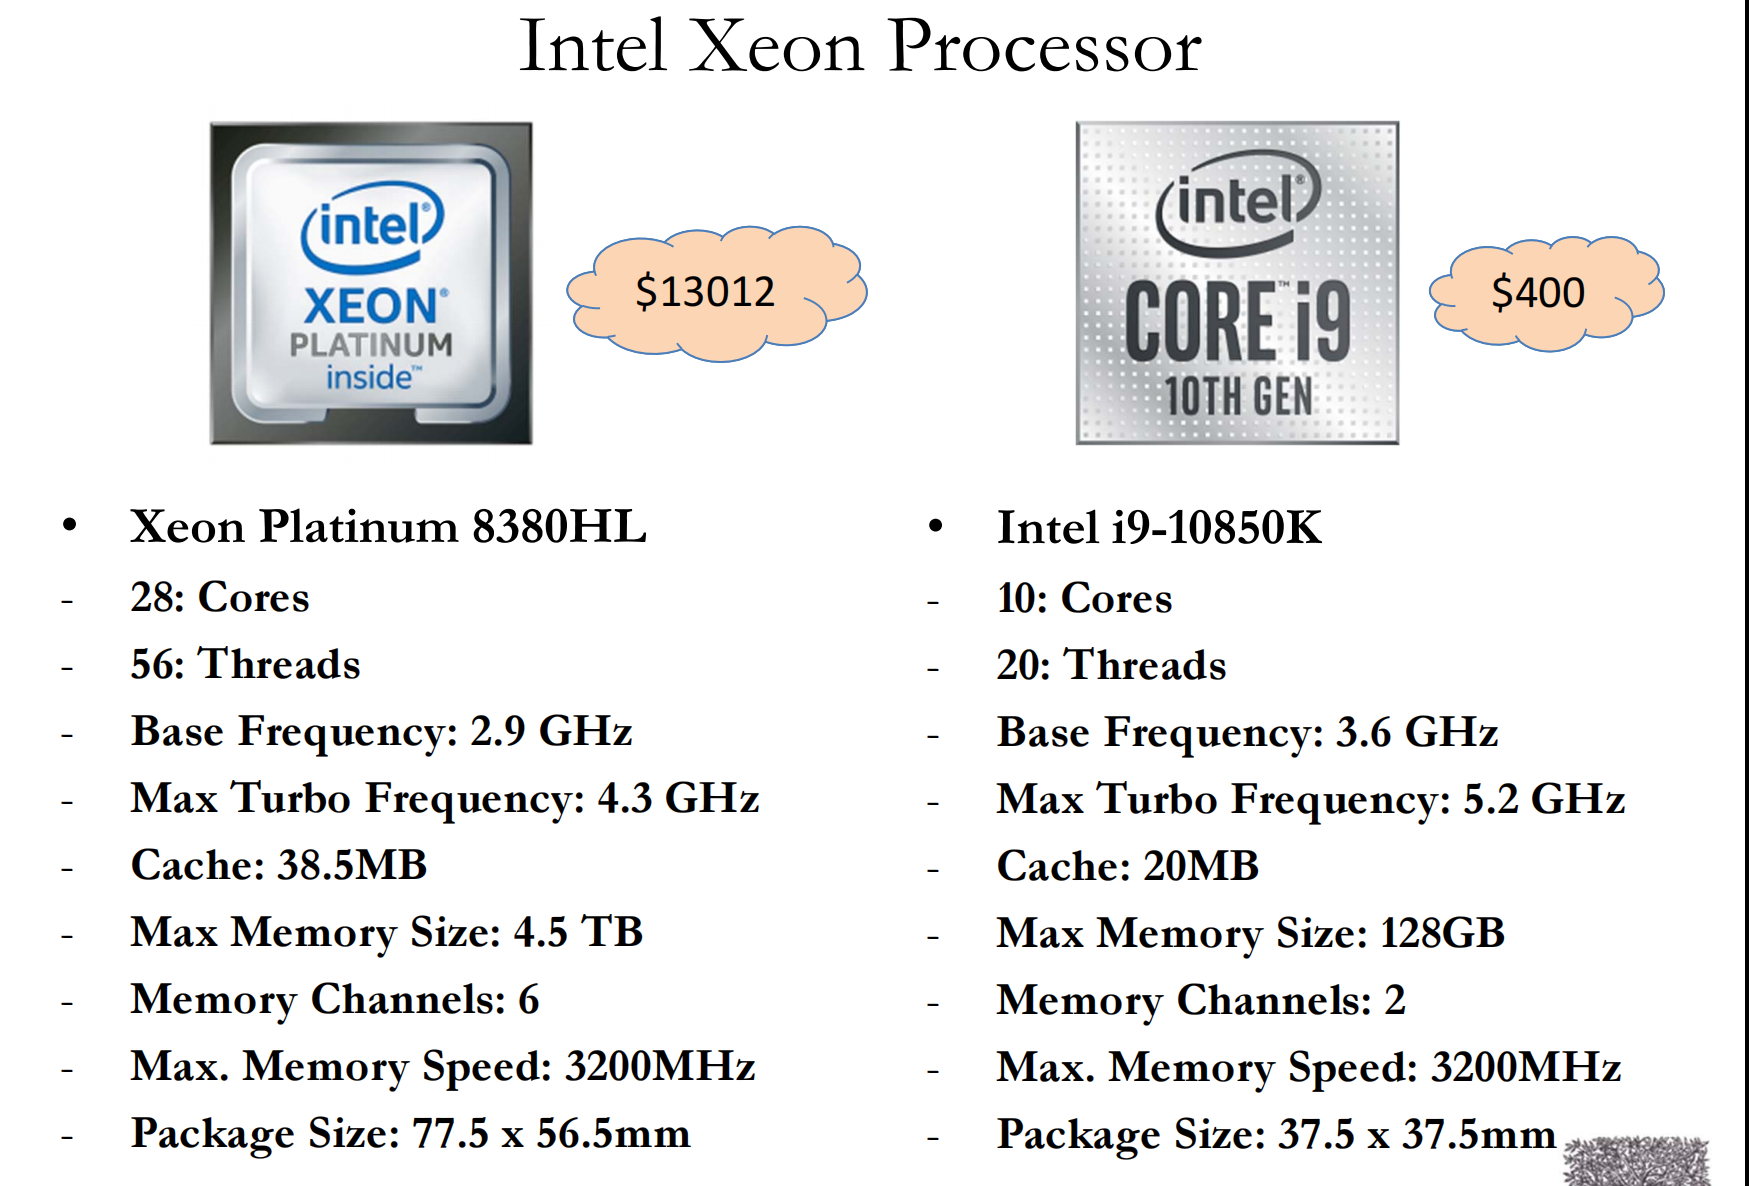
\includegraphics[width=\textwidth]{ProcessorOverview.png}
\subsection{Why the prices of two processors differs?}
\begin{enumerate}
    \item The prices increase exponentially as the number of Cores and Threads increase. That's because every core has a bad possibility, so the difficult of making a processor with many cores much harder.
    \item Significant: The memory Chaneels of XEON is three times by i9, which means it has three times as many pins as i9 has.
\end{enumerate}

\section{Digital Design}
\subsection{Abstraction}
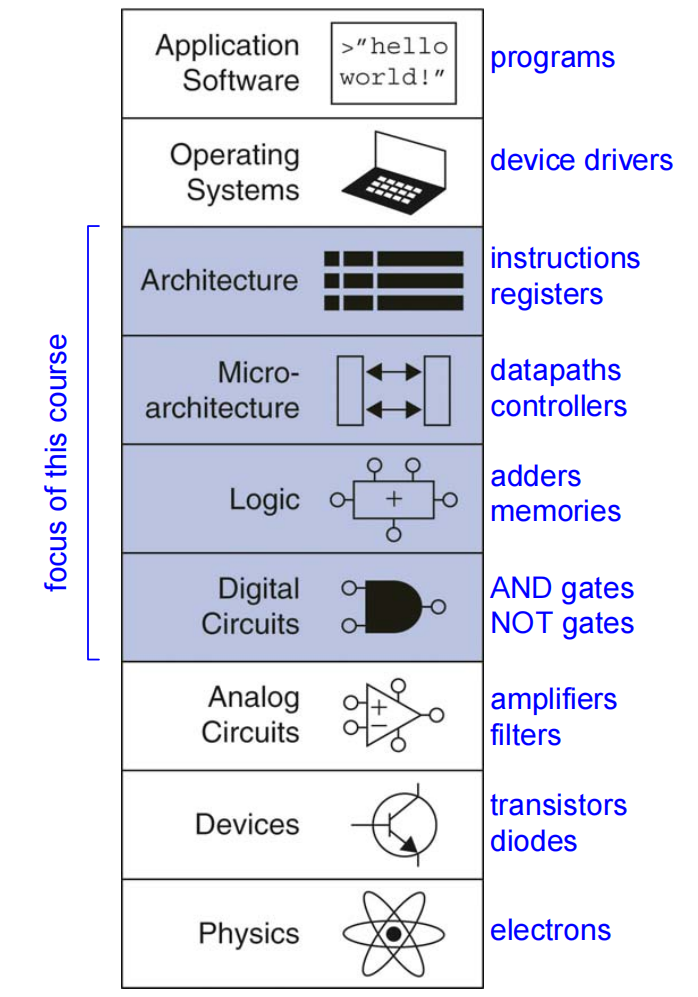
\includegraphics[width=0.6\textwidth]{Abstraction.png}
\subsection{The Digital Abstraction}
\begin{itemize}
    \item Most physical variables are continuous \begin{itemize}
        \item Voltage on a wire
        \item Frequency of an oscillation
        \item Position of a mass
    \end{itemize}
    \item Digital abstraction considers discrete subset of values
\end{itemize}
\subsection{Digital Discipline: Binary Values}
\begin{itemize}
    \item Two discrete Values: \begin{itemize}
        \item 1's and 0's
        \item 1, true, high
        \item 0, false, low
    \end{itemize}
    \item 1 and 0: voltage levels, rotating gears, fluid levels
    \item Digital circuits use voltage levels to represent 1 and 0
\end{itemize}
\subsection{Decimal to Binary Conversion}
Method: repeatedly divided by 2, remainders goes in next most significant bit
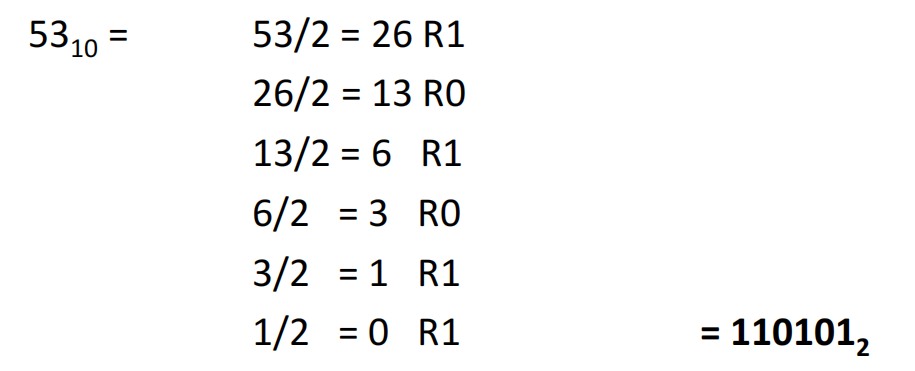
\includegraphics[width=\textwidth]{DecimalToBinary.png}
\subsection{Signed Binary Numbers}
\subsubsection{Sign/Magnitude Numbers}
Problems
\begin{itemize}
    \item Has two 0 values, positive 0 and negative 0
    \item Addition of a negative and a postive will fail
\end{itemize}
\subsubsection{Two's Complement Numbers}
Conversion from positive to negative:
\begin{itemize}
    \item Invert every bit
    \item Add 1
\end{itemize}
\subsection{Logic Gates}


\end{document}